\documentclass{article}
\usepackage{graphicx}

\usepackage{setspace}
\doublespacing
%\onehalfspacing
\usepackage[spanish]{babel}
\selectlanguage{spanish}
\usepackage[utf8]{inputenc}

\usepackage{fancyhdr}
\pagestyle{fancy}

\usepackage{xcolor}

\usepackage{lipsum}
\setlength\headheight{40pt} %% just to make warning go away. Adjust the value after looking into the warning.
% \rhead{{\color{blue}\rule{1cm}{1cm}}}
\fancyhf{}
\rhead{
\includegraphics[width=7cm]{logo}}


\title{Servicio Especializado de Sistematizaci\'{o}n de Registros y Sistemas de V\'{i}ctimas de Trata de Personas\\
\vspace{200px}
{\bf PLAN DE TRABAJO}}


\author{\vspace{75px}Dr. Jos\'{e} Manuel Magallanes, Ph.D}
\date{17 de Noviembre de 2017}
\usepackage{Sweave}
\begin{document}
\Sconcordance{concordance:PlanDeTrabajo.tex:PlanDeTrabajo.Rnw:%
1 29 1 1 0 93 1}

\maketitle
\thispagestyle{empty}

%#############
\clearpage
\setcounter{page}{1}
\section{Presentaci\'{o}n}

El servicio contratado busca tener datos integrados de v\'{i}ctimas de \emph{la trata de personas}.   La integraci\'{o}n se har\'{a} en base a los registros de distintos sistemas que contengan informaci\'{o}n de estas v\'{i}ctimas. Las v\'{i}ctimas pueden tener informaci\'{o}n hist\'{o}rica.

La finalidad del trabajo es que, a partir de los datos integrados, se pueda identificar los lugares donde tal actividad il\'{i}cita se lleve a cabo con mayor incidencia, en relaci\'{o}n a los dem\'{a}s lugares identificables del pa\'{i}s. 

\section{Insumos requeridos}

A fin de llevar a cabo este trabajo, es necesario que la Dirección General de Seguridad Democr\'{a}tica del Ministerio del Interior, o alguna oficina alternativa que designe \'{e}sta, provea los datos provenientes de:

\begin{enumerate}
\item Sistema de Registro y Estad\'{i}stica del delito de Trata de Personas y afines (RETA), que contienen informaci\'{o}n de la investigaci\'{o}n de delitos de trata a nivel policial.  

\item Sistema de Informaci\'{o}n Estrat\'{e}gica sobre Trata de Personas (SISTRA), informaci\'{o}n de la investigaci\'{o}n de delitos de trata de personas en el Ministerio P\'{u}blico.

\item Sistemas de denuncias e informaci\'{o}n policial (SIDPOL y ESINPOL), sobre denuncias formuladas ante comisar\'{i}as y unidades especializadas.

\item Registros  de denuncias y/o investigaciones seguidos a nivel del Ministerio de Justicia (MINJUS).

\item Registros de atenci\'{o}n de v\'{i}ctimas de trata en Centros de Emergencia Mujer, del Ministerio de la Mujer y Poblaciones Vulnerables (MIMP).

\item Registros de atenci\'{o}n de v\'{i}ctimas de trata de los Centros de atenci\'{o}n Residencial del MIMP
\end{enumerate}

Estos datos no son de libre acceso, por lo que s\'{o}lo personal autorizado puede solicitarlo.

\section{Limitaciones del Trabajo}

De la secci\'{o}n anterior se desprende que el consultor no puede iniciar su trabajo si el cliente desde el MINITER no nos proporciona oportunamente los insumos.

\section{Actividades de la Consultor\'{i}a}

Este trabajo consta de una serie de pasos. La secuencia a seguir va desde el almacenamiento hasta la detección de patrones\cite{magallanes_reyes_introducing_2017}. Estas etapas se describen a continuación.

\subsection{Almacenamiento de la Datos}

Los datos entregados por el cliente del MININTER será colectados y almacenados en un repositorio. Según el tamaño de los archivos entregados, los datos serán almacenados en repositorios tales como \emph{Box}, \emph{Dropbox}, \emph{Github} o \emph{AmazonWS}. Los repositorios serán sólo temporales, es decir, se existirán mientras dure el trabajo. La manipulación de los Datos se hará usando diversos programas, tales como R y Python, sin descartar el uso de SPSS y/o STATA. Ni el uso de repositorios, ni el tipo de programas estadísticos a utilizar generarán gastos adicionales al cliente del MININTER, ni generarán excusa de ningún tipo para demorar los entregables del trabajo.

\subsection{Preparación de los Datos}

Los datos, antes de ser analizados, pasarán por una serie de pasos, cada uno de ellos con diversa duración. Así tenemos:

\subsubsection{Identificación de Escalas}
Los valores a entregar pueden estar en diversos tipos de escalas, usándose para este caso la clásica diferenciación: \emph{nominal}, \emph{ordinal}, \emph{intervalo} y \emph{razón} \cite{stevens_theory_1946}. Sabiendo en qué tipo de escala está una variable en particular, sabremos qué técnicas debemos elegir para los cálculos y visualizaciones posteriores. Al final, se habrá identificado la escala de cada variable, pero aun no se formateará pues primero habrá que verificar si los datos están \emph{limpios}.

\subsubsection{Limpieza de valores}

Una vez identificada la escala de las variables (columnas) se procederá a verificar que los valores de cada celda estén no contengan caracteres que alteren los cálculos. Este es uno de los procesos más tediosos. Al final, se tendrán valores verificados y confiables.

\subsubsection{Formateo de valores}
Los datos limpios deben ser justamente transformados para que los programas estadísticos los reconozcan en la escala respectiva. Al final, se tendrá data con el formato que los programas reconocerán.

\subsubsection{Integración de Datos}
En esta etapa se integrará los datos de todas las tablas. Sólo se podrá integrar las tablas que tengan un campo \emph{clave} común que permita la integración o \emph{merge}. Si alguna tabla no tuviera campos en común, será tratada de manera individual, y se evaluará como esos datos contribuyen al análisis posterior. Al final se tendrá una tabla única con todas las tablas integrables.

\subsubsection{Formateo de Datos}
La data integrada podría necesitar formato diferente al de una tabla de datos clásica (resultado anterior). Al final, se tendrá la data integrada en el formato adecuado, entre los cuáles pueden ser: panel, serie temporal, red, data de sobrevivencia, existe la posibilidad de algún formato no convencional (\emph{NoSQL}).

\subsection{Análisis de Datos}

Esta etapa permitirá conocer qué se tiene. Aquí comienza la etapa de exploración de la data integrada formateada; lo cual permite hacer análisis posteriores mucho más complejos.

\subsubsection{Análisis Exploratorio}

La exploración de datos permite saber cómo se comporta cada variable. El comportamiento sugiere la distribución de probabilidad que esta produciendo tales datos, las técnicas multivariadas dependen de saber tales distribuciones para justamente saber cómo estimar los parámetros de la población. En caso la distribución no fuese fácilmente identificable, deberemos utilizar técnicas \emph{no paramétricas}\cite{hollander_nonparametric_2014}.

\subsubsection{Análisis Multivariado}
El análisis multivariado permitirá saber qué tanto podemos organizar los casos usando toda o la mayor parte de la información disponible, y qué tanto podemos reducir la alta dimensionalidad de las variables originales en tres o dos dimensiones. Al final, la data integrada estará lista para seber qué indicadores compuestos se podrán proponer y calcular.

\subsection{Detección de Patrones}
\subsubsection{Creación de Indicadores}
Luego del análisis multivariado, podemos proponer los indicadores compuestos adecuados. Los indicadores serán calculados cambiando la unidad de análisis; es decir, considerando que la data integrada tiene en cada fila a una \emph{persona}, éstas serán agregadas en una unidad geográfica comprehensiva. De esta manera, los indicadores serán a nivel geográfico. 

\subsubsection{Minería de la Incidencia}
La minería consiste en encontrar patrones y casos atípicos entre los indicadores. Según el tipo con los que se cuente, podremos encontrar diversos patrones a nivel nacional. Al final, se podrá producir la información requerida por el cliente del MINITER, saber dónde hay mayor incidencia.

\section{Cronograma}

Considerando el 14 de noviembre como el inicio de este trabajo (fecha de recepción de este trabajo), el cronograma, basado en semanas de cinco dias, es el siguiente:

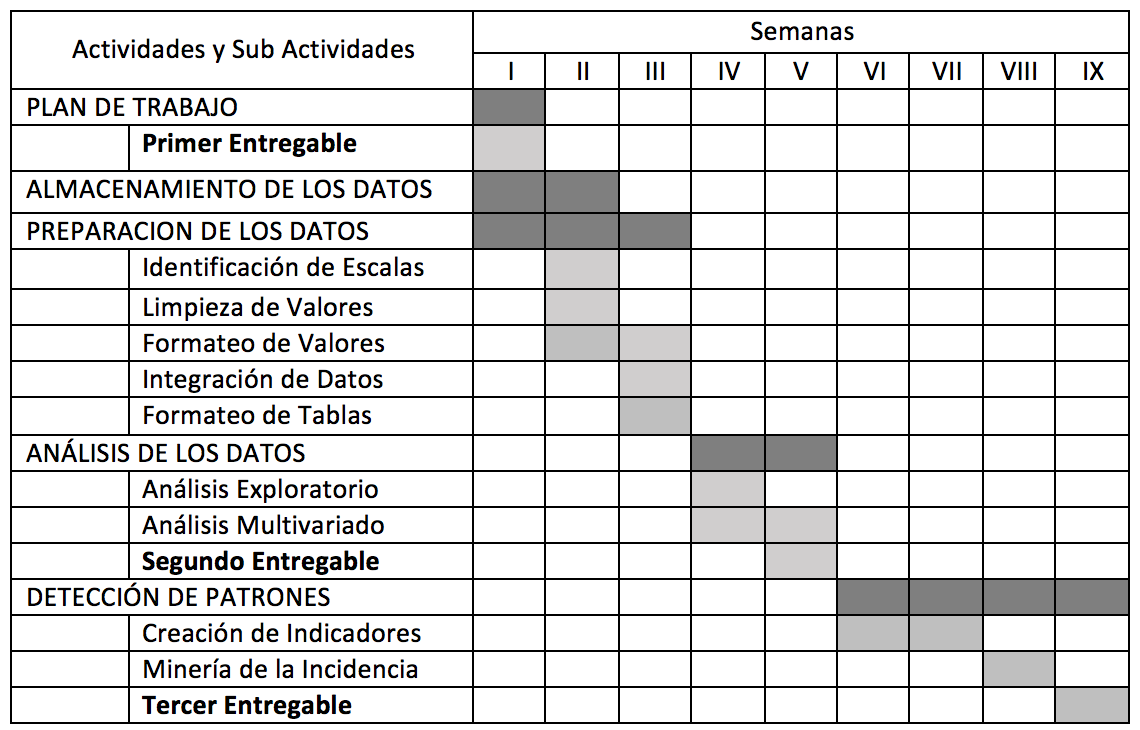
\includegraphics[width=\textwidth]{cronograma}

\bibliographystyle{unsrt}
\bibliography{Mininter_4031_e1}

\end{document}
